\bookchapter{第三十七章：范式革命——从“写代码”到“指挥AI写代码”}

\chapterintro{恭喜你，翻开这本书的你，正站在一场职业范式革命的正中央。这场革命的起点，是 2025 年一个程序员在社交媒体上发的一句话。听起来有点戏剧性？但事实就是这样。}

\booksection{一、Vibe Coding 的诞生：一句话引发的运动}

2025 年 2 月，Andrej Karpathy——这个名字请先记住，后面还会见到他好几次——在社交媒体上发了一条后来被反复引用的推文：“有一种新编程方式叫\textbf{Vibe Coding}，你完全凭感觉（vibes）来，忽略代码细节，让 AI 包揽一切。你看到什么就说什么，复制粘贴，基本上能用就行。”

这条看起来随口一说的发言，其实精准命名了一场已经悄然发生的范式转移：\textbf{人类不再逐行编写代码，而是用自然语言描述意图，由 AI 完成实现}。Karpathy 的措辞带着一丝戏谑，但背后是个深刻的洞察：当 AI 的代码生成能力跨过某个阈值之后，编程的瓶颈就不再是“这行代码我能不能写出来”，而是“这件事我到底想不想得清楚”。

\begin{tcbinfo}{小贴士：Vibe 是什么？}
Vibe 直译是“氛围、感觉”。Vibe Coding 就是“跟着感觉指挥 AI 编程”——你描述想要什么，AI 负责实现。记住这个词，它是这场革命的“出生证明”。

\end{tcbinfo}

从那一刻起，“编码”这个词的含义开始分裂：传统的编码是把\emph{设计}翻译成\emph{语法}；新的编码是把\emph{意图}翻译成\emph{指令}。前者考验手指，后者考验脑子。

Vibe Coding 这个词很快从戏谑变成了严肃的工程概念。到 2026 年中期，它已经从一个社交媒体上的梗，演化为一套完整的方法论体系——涵盖需求表达、上下文管理、迭代验证到质量保障的全流程。人们也意识到：\textbf{“凭感觉”只是入门阶段的状态，真正高效的 AI 编程需要一套系统化的思维方式}。而这套思维方式，就是本书要给你的东西。

\booksection{二、2026 年现状：Agentic Engineering 时代}

到了 2026 年 8 月，AI 编程领域已经经历了几次重要的范式迭代。Vibe Coding 是最初的火花，但很快大家发现：光“凭感觉”和 AI 聊天，产出的代码质量极不稳定——有时惊艳，有时翻车。于是范式开始进化：\textbf{从简单的对话式编程，走向结构化的 Agent 工程}。

又是 Karpathy，2026 年初提出了\textbf{Agentic Engineering}的概念。与 Vibe Coding 的“说了就生成”不同，Agentic Engineering 强调：给 AI 一个目标，让它\emph{自主规划步骤、调用工具、验证结果、迭代修正}。AI 不再只是一个代码生成器，而是一个能感知环境、做出决策、执行动作的智能体（Agent）。

这个转变带来了三个关键变化：

\begin{enumerate}
  \item \textbf{交互模式变了}：从"一问一答"变成"设定目标后放权"。
  \item \textbf{工作产物变了}：从"一段代码"变成"一个完整的项目"。
  \item \textbf{人的角色变了}：从"逐行审核代码"变成"定义边界、验收结果"。
\end{enumerate}

数字不会说谎：Cursor 在 2026 年 4 月发布的 Cursor 3 版本中，\textbf{Agent 模式的使用率首次反超 Tab 补全模式}，标志着开发者已经大规模转向这种工作方式；而 Claude Code 这个终端原生的 AI 编程工具，到 2026 年中期已达到年化收入 25 亿美元的规模。下面的趋势图能让你直观感受这个交叉时刻：

\begin{center}
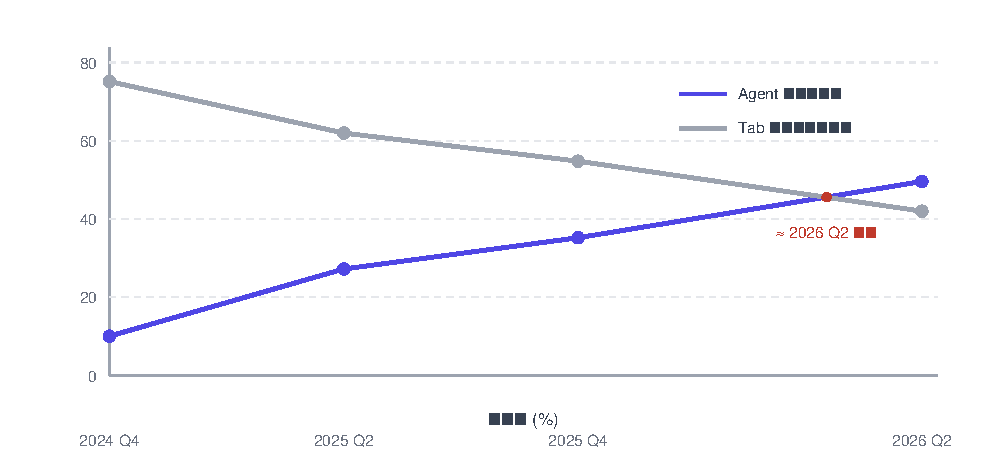
\includegraphics[width=0.92\linewidth]{figures/fig-di-san-shi-qi-zhang-1}
\\[2pt]\small 图 1：AI 编程交互模式使用率变化趋势（基于行业调研数据估算，2026 Q2 Agent 模式反超 Tab 补全）
\end{center}

但说句实在话：工具和模型的变化只是表象。\textbf{无论你用 Cursor 还是 Claude Code，无论底层模型是 GPT-5 还是 Claude 4.5，成功的 AI 编程实践者都在遵循同一套底层方法论}。这就是本指南要教给你的东西。

\booksection{三、核心认知转变：从 Coder 到 Conductor}

传统编程教育教你如何成为一个 Coder——理解语法、记忆 API、调试逻辑错误。AI 编程时代，这个角色正在被重新定义。你不再需要亲手把每一行代码写出来，但你需要成为一个“指挥官”（Conductor）：\textbf{定义战场、制定规则、分配任务、验收成果}。

这个转变的核心不在于“你会不会写代码”，而在于“你会不会想清楚要做什么”。一个优秀的指挥官不一定是最好的士兵，但他必须最清楚战役的目标、地形和兵力部署。同理，一个优秀的 AI 编程实践者不一定精通每一种编程语言的语法细节，但他必须最清楚项目的目标、架构约束和质量标准。

这张表值得你多看两遍——它概括了这次角色转变的全部内涵：

\begin{center}
\begin{tabularx}{\linewidth}{|X|X|X|}
\hline
\textbf{维度} & \textbf{传统 Coder} & \textbf{AI 指挥官（Conductor）} \tabularnewline
\hline
核心技能 & 语法记忆、API 调用、调试 & 需求定义、上下文管理、验收判断 \tabularnewline
工作方式 & 逐行编写代码 & 描述意图，审查产出 \tabularnewline
质量把控 & 自己写的，自己心里有数 & 通过测试和审查验证 AI 产出 \tabularnewline
知识要求 & 深度掌握特定语言/框架 & 广度理解技术全貌，深度理解业务逻辑 \tabularnewline
瓶颈所在 & 编码速度和语法记忆 & 思考清晰度和表达能力 \tabularnewline
错误来源 & 语法错误、逻辑遗漏 & 需求模糊、上下文不足 \tabularnewline
\hline
\end{tabularx}
\end{center}

\begin{center}\small\color{gray}传统 Coder 与 AI 指挥官的能力维度对比\end{center}

这绝不是说编程知识不重要了。恰恰相反：当你能看懂 AI 写的代码时，你才能有效地审查和修正它；当你理解数据结构和算法时，你才能判断 AI 的方案是否合理。\textbf{知识储备决定了你的“指挥上限”——但知识的角色从“执行工具”变成了“判断依据”}。

\booksection{四、为什么方法论比工具更重要}

工具每三个月迭代一次，方法论每三年才进化一次。学会一个工具的操作，三个月后可能就过时了；掌握一套思维方式，三年后依然适用。

很多人在入门 AI 编程时，第一件事就是追问“哪个工具最好”“哪个模型最强”。这些问题不是不重要，但它们问错了优先级。2026 年 8 月的工具格局和 2025 年 8 月已经完全不同——Trae、Qoder 等工具兴衰起伏，Cursor 从插件变成了独立 IDE 又进化到 Cursor 3，Claude Code 从实验性项目变成了终端编程的主流选择。但在这剧烈变化背后，\textbf{成功实践者遵循的思维原则几乎没有改变}。

这就是为什么本书不会把篇幅花在教你某个工具的具体操作上——那些内容写完就会过时。相反，本书的全部重心放在一套经过验证的思维方法论上：如何思考需求、如何与 AI 沟通、如何验证产出、如何持续迭代。\textbf{掌握了这套方法论，你换任何工具都能快速上手；只学了工具操作，换一个工具就要从零开始}。

\begin{tcbinfo}{给零基础读者的定心丸}
如果你是零基础，别被“方法论”三个字吓到。方法论不是抽象的哲学，它就是一套“遇到问题该怎么想”的操作手册。就像学做菜：你可以照着菜谱一步步来（工具操作），但真正的大厨理解的是“为什么要这样调味”“火候怎么控制”（方法论）。本书会从最基础的概念讲起，每个原则都配具体的对比案例，确保你不仅理解“是什么”，更能掌握“怎么做”。

\end{tcbinfo}

\begin{tcbpractice}{来动手：给现在的你拍张"角色照"}
拿出一张纸，写下三个问题的答案：(1) 你现在是怎么用 AI 帮你写代码的（如果用过的话）？(2) 你更像上表中的“Coder”还是“指挥官”？(3) 你希望三个月后的自己会怎样描述自己的工作方式？写完后夹在书里，读完第四十七章再回来看——你会发现变化比想象中快。

\end{tcbpractice}

\begin{tcbsummary}{本章小结}
\begin{itemize}
  \item 2025 年 Karpathy 用"Vibe Coding"命名了 AI 编程革命：从逐行写代码，变成用自然语言描述意图
  \item 2026 年进化到 Agentic Engineering：给目标、放权、AI 自主规划执行，人负责验收
  \item Cursor 3 的 Agent 模式使用率首次反超 Tab 补全；Claude Code 年化收入达 25 亿美元
  \item 你的新角色是 Conductor（指挥官）：定义战场、制定规则、分配任务、验收成果
  \item 工具每三个月迭代一次，方法论每三年才进化一次——学方法论，不学操作
\end{itemize}

\end{tcbsummary}
